\documentclass{oxmathproblems}
\usepackage{graphicx}
\usepackage{hyperref}
\usepackage{footmisc}
\usepackage{listings}
\usepackage{color}
\usepackage{xcolor}
\graphicspath{{imagenes/}} 

\course{EE447 Mobile Internet HW 2 \\The Double Spend Problem}

\newtheorem{theorem}{Theorem}
\newtheorem{lemma}[theorem]{Lemma}
\newtheorem{proposition}[theorem]{Proposition}
\newtheorem{corollary}[theorem]{Corollary}
\newtheorem{exercise}{Exercise}
\newtheorem{definition}{Definition}
\theoremstyle{definition}
\lstset{
	keywordstyle=\color{blue!70}\bfseries, %设置关键词为蓝色,需要引xcolor宏包
	basicstyle=\ttfamily\footnotesize, 
	commentstyle=\ttfamily, %基本和注释的字体都使用默认的等宽,而非texlive调用的中文字体
	showstringspaces=false, %不显示中间的空格
	frame=shadowbox,
	rulesepcolor=\color{red!20!green!20!blue!20},
}
\makeatletter \renewenvironment{proof}[1][Proof] {\par\pushQED{\qed}\normalfont\topsep6\p@\@plus6\p@\relax\trivlist\item[\hskip\labelsep\bfseries#1\@addpunct{.}]\ignorespaces}{\popQED\endtrivlist\@endpefalse} \makeatother
\makeatletter
\renewenvironment{solution}[1][Solution] {\par\pushQED{\qed}\normalfont\topsep6\p@\@plus6\p@\relax\trivlist\item[\hskip\labelsep\bfseries#1\@addpunct{.}]\ignorespaces}{\popQED\endtrivlist\@endpefalse} \makeatother

\begin{document}
\begin{center}
	% Please write down your name, student id and email.
	Name: Hongjie Fang \quad Student ID:518030910150 \quad Email: \href{mailto:galaxies@sjtu.edu.cn}{galaxies@sjtu.edu.cn}
\end{center}
\textbf{Problem}\footnote{Translated by DeepL Translator: \url{https://www.deepl.com/translator}}.

Assume that the longest chain of a blockchain acknowledges every block received. Due to the longest chain principle of the blockchain, the confirmed blocks on the chain may be discarded due to the extension of other branches, making the digital assets contained in the block potentially consumed repeatedly. This is a common double-spending problem in blockchain. To cope with this problem, the concept of "$k$-confirmed transaction" is proposed, which means that a transaction is officially completed only after it has received $k$ confirmations from the blockchain.

After a transaction is confirmed, an attacker attempts to cause the transaction to be discarded by creating a branch chain. The cost per unit of time for the attacker to obtain 51\% of the network-wide computing power in the blockchain is \$10,000, and the probability that 51\% of the network-wide computing power successfully generates a block on the target branch per unit of time is 5\% (if the attacker succeeds in generating a block per unit of time, it is considered that the branch chain adds a new block and no new block is generated on the main chain; if the attacker fails in generating a block per unit of time, it is considered that the branch chain adds no new block and no new block is generated on the main chain). If the attacker fails to generate a block per unit of time, the branch chain is considered to have not added a new block and someone else has successfully generated a block on the main chain). There is a transaction worth \$1,000,000 that is formally completed after $k$ confirmations. What is the minimum size of $k$ to ensure that the expected cost of the transaction to be successfully tampered with by an attacker using 51\% of the computing power is higher than the amount of the transaction?

\begin{solution}
	In general, we assume that the probability that the attacker successfully generates a block on the target branch per unit time is $p$, the cost per unit time for the attacker is $c$, and the target transaction is worth $w$. We are going to calculate the expected cost of transaction to be successfully tampered with by an attacker.

	To successfully tamper with the blcokchain, the generated branch needs to have at least one more block than the branch that contains real transaction. Initially, the main branch that contains real transaction has $(k + 1)$ blocks more than the attack branch, including $k$ comfirmation blocks and one transaction block. So the attacker needs to generate $(k + 2)$ extra blocks in the attack branch more than the number of blocks generated during this period in the main branch. The whole attacking process is illustrated in Fig. \ref{fig1}.
	\begin{figure}[htbp]
		\centering
		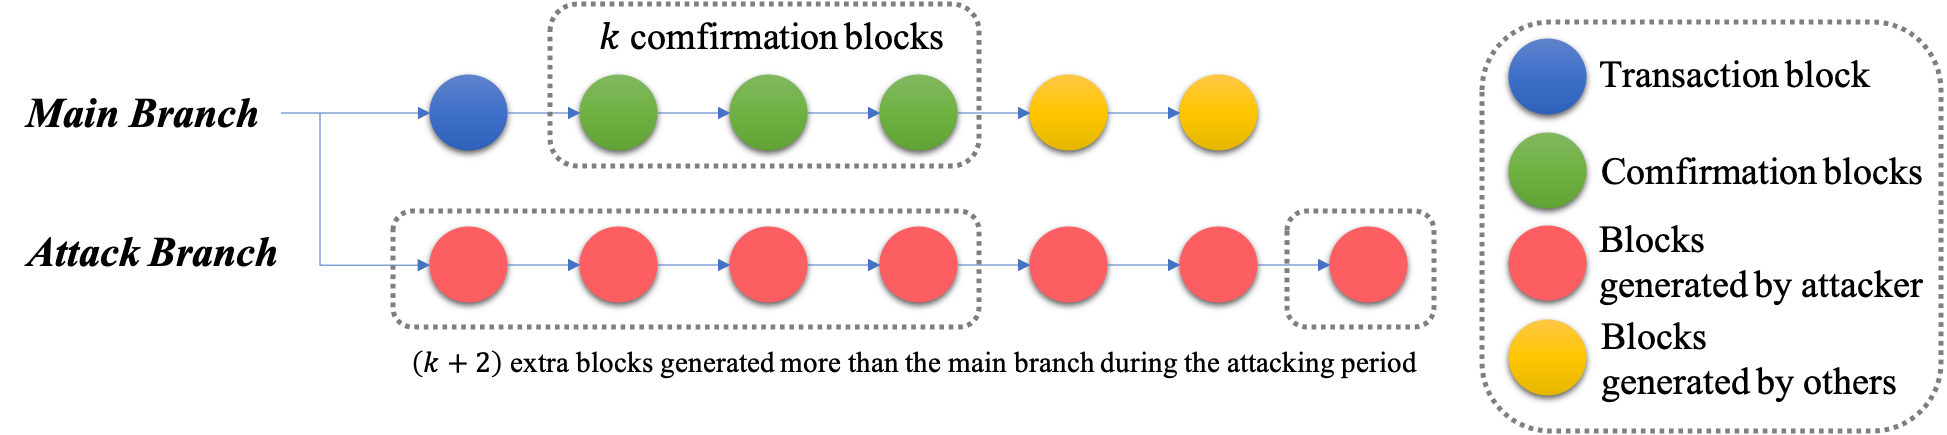
\includegraphics[width=\linewidth]{1.png}
		\caption{The whole attacking process}
		\label{fig1}
	\end{figure}

	Apart from the extra blocks in the attack branch, we assume that in both branches, $x$ blocks are generated during the attacking process. Therefore, totally $(k + 2x + 2)$ blocks are generated during the attacking process. Suppose the probability that $x$ blocks are generated in both branches during the attacking process is $P(x)$. Hence,
	$$
	P(x) = \left(\begin{matrix}k+2x+2 \\ x\end{matrix}\right) p^{k+x+2} (1-p)^x - \sum_{y=0}^{x-1} P(y) \left(\begin{matrix}2(x - y) \\ x - y\end{matrix}\right)p^{x-y}(1-p)^{x-y} \quad (x \ge 1)
	$$
	where $\left(\begin{matrix}n \\ k\end{matrix}\right)$ is the combination number of parameters $n$ and $k$. Initially, $P(0) = p^{k+2}$.
	
	Now, let us explain the formula in details.
	\begin{itemize}
		\item The first term is the probability that $x$ blocks are generated in both branches when totally $(k+2x+2)$ blocks are generated. Notice, the attacking process may already end previously because the attacking branch may already have $(k + 2)$ blocks more than the making branch.
		\item The second term will subtract the probability that $x$ blocks are generated in both branches when totally $(k+2x+2)$ blocks are generated, but the attacking process is already end, from the total probability calculated in the first term. Therefore, we enumerate when the process finishes, \textit{i.e.}, the variable $y$. For those situations, we just need to simulate the generating process $2(x-y)$ times further, and during this time, both branches generate $(x - y)$ blocks. 
	\end{itemize}

	Therefore, the expected cost of successfully attacking is:
	$$
	E(cost) = \sum_{x=0}^\infty P(x) \cdot (k+2x+2)c
	$$

	And we just need to find out the minimum $k$ such that
	$$
	E(cost) = \sum_{x=0}^\infty P(x) \cdot (k+2x+2)c > w
	$$

	Since the formula includes infinite summation, and it is difficult to derive the close form solution to $P(x)$, we write a program to give the numerical solution. Since it may take long to convergence, and the value of the combination numbers may be extremely large. We use linear regression to predict $P(x) \cdot (k + 2x + 2) \cdot c$ for large $x$, until this term reaches negative.
\begin{lstlisting}[language=python]
def calc_expected_cost(k, p, c):
    '''
    Calculate the numerical value of expected cost when given k, p and c.

    Parameters
    ----------
    k, p, c: the given parameters, explained previously in the solution.
    
    Returns
    -------
    The numerical value of expected cost.
    '''
    E = 0
    P = []
    D = []
    x = 0
    while True:
        Px = comb(k + x + x + 2, x) * pow(p, k + x + 2) * pow(1 - p, x)
        if x > 0:
            for y in range(x - 1):
                Px = Px - P[y] * comb(2 * (x - y), (x - y)) 
                               * pow(p, x - y) * pow(1 - p, x - y)
        if Px == np.inf:
            break
        P.append(Px)
        delta = Px * (k + x + x + 2) * c
        D.append(delta)
        E += delta
        x += 1
    
    reg = LinearRegression()
    reg.fit(np.array(range(x - 100, x)).reshape(-1, 1), D[len(D) - 100:])

    while True:
        delta = reg.predict(np.array([x]).reshape(1, -1))[0]
        if delta < 0:
            break
        E += delta
        x += 1
    return E 
\end{lstlisting}
	Set $p = 0.51$, $c = 1$ (unit: \$10,000), and enumerate $k$ then execute the program, we can list the influence of $k$ on the expected cost as follows.
	\begin{table}[htbp]
		\centering
		\caption{The influence of $k$ on the expected cost $E(cost)$}
		\label{tab1}
		\begin{tabular}{|c|c|c|c|}  
			\hline  % 表格的横线
			$k$ & $E(cost)$ (unit: \$10,000) & $k$ & $E(cost)$ (unit: \$10,000)\\ \hline
			0 & 44.78934262241547 &10 & 306.67805412101393 \\
			1 & 73.84332272554721 &11 & 330.5734107375575 \\
			2 & \textbf{102.10130199424312} &12 & 354.03950302354417 \\
			3 & 129.73732618945058 & 13 & 377.84293299662426 \\
			4 & 156.59278841516797 & 14 & 401.45768077718634 \\
			5 & 182.95282187095157 & 15 & 425.7710396374425 \\
			6 & 208.56668084212004 & 16 & 450.26824220324215 \\
			7 & 233.8359965147291 &17 & 475.955250947649 \\
			8 & 258.4203552586561 & 18 & 502.41497625543695\\
			9 & 282.84179355170596 &19 & 530.7735112002084 \\ \hline	
		\end{tabular}
	\end{table}
	\begin{figure}[htbp]
		\centering
		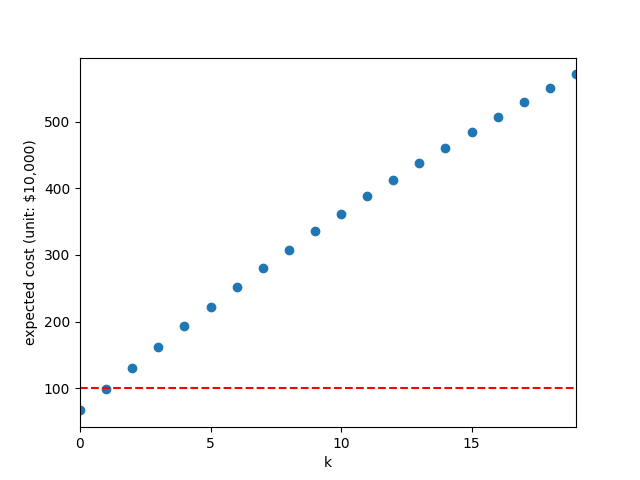
\includegraphics[width=0.7\linewidth]{2.png}
		\caption{The influence of $k$ on the expected cost $E(cost)$}
		\label{fig2}
	\end{figure}

	From Tab. \ref{tab1} and Fig. \ref{fig2} we can see that when $k = 2$, $E(cost) \approx \$102101 > \$100000 = w$. Hence, we choose $k = 2$ as our answer.

	Now, let us interpret the answer in a more intuitive way. According to the setting of the problem, the attack branch of attacker takes 49\% blocks while others takes 51\% blocks when given a certain number of blocks. From the attacker's view, the success of attack needs
	$$
	\frac{1 + 2\%}{2}x - \frac{1 - 2\%}{2}x > k + 1
	$$
	Notice here we use $> k + 1$ instead of $\ge k + 2$ because in the meaning of expectation, we need continuous variables instead of discrete variables. Also, the attacker know that his/her profit must be non-negative, which indicates $x \leq 100$ according to the setting of the problem. Therefore, the critical value for successful attacking is $k = 1$. Hence, we need to set at least $k = 2$ to prevent attacking according to the configuration of the problem.

	In conclusion, the minimum size to ensure that the expected cost of the transaction to be successfully tampered with by an attacker using 51\% of the computing power is higher than the amount of the transaction is $k = 2$.
\end{solution}

\end{document}
